\vspace{-6pt}
\mysection{Description de la solution}

\mysubsection{Choix du robot}

Pour choisir le robot le plus adéquat pour notre solution, on doit prendre en compte le domaine d’application du robot, la cadence de production, la charge que le robot doit supporter et le rayon d’action.
Dans notre cellule robotique, l’application du robot est palettiser les cartons dans les palettes.On choisit un robot du type palettisation: modèles M-710iC/50H, R-1000iA/80H, R-2000iB/100H et M-410.
La charge embarquée maximale du robot est composée du préhenseur plus le carton. Le préhenseur a une masse de 20 $ kg $, de centre de gravité (CDG) (0, 0, 60) en millimètres. Les inerties sont $ L_{xx} = 8.54 \times 10^{-1}$  $ kg.m^2 $, $ L_{yy} = 3.04 \times 10^{-1}$  $ kg.m^2 $ et $ L_{zz} = 1.083 kg.m^2 $. Ces sont les données à vide, exprimés dans le repère dont l'origine est située au centre de la platine du robot, l’axe Z est perpendiculaire et sors de la platine et l’axe X point vers le haute quand le robot est sur ses zéros mécaniques. On l’appelle repère R1.
Chaque carton a une masse de 50 $ kg $ et ils sont considérés comme des solides homogènes. Les dimensions sont $ 780 \times 540 \times 350 $ $ mm $, donc son CDG coïncide avec le centre géométrique. Par rapport à un repère situé au centre du carton (repère R2), comme montre la figure \ref{fig:Repere_carton} les inerties sont $ L_{xx} = 1.725 $  $kg.m^2 $, $ L_{yy} = 3.045$  $ kg.m^2 $ et $ L_{zz} = 3.75$  $ kg.m^2 $.
Quand le préhenseur est en charge, le robot doit supporter une masse de 70 $ kg $. On considère que le centre géométrique du carton est situé sur l’axe Z du repère R1. Le CDG par rapport à ce même repère est (0, 0, 214) $ mm $ et les inerties sont $ L_{xx} = 6.360 kg.m^2 $, $ L_{yy} = 7.130 $  $kg.m^2 $ et $ L_{zz} = 4.833 $  $kg.m^2 $.

\begin{figure}[H]
	\begin{center}	
		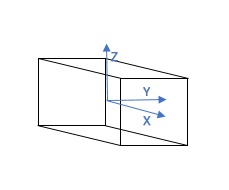
\includegraphics[width=8cm]{Description_de_la_solution/Repere_carton.jpg}
		\caption{Repère R1 au centre du carton}
		\label{fig:Repere_carton}
	\end{center}
\end{figure}
\pagebreak
Pour déterminer le rayon d’action minimal pour le robot dans cette application, au début on a besoin de fixer une disposition a priori des \textit{fixtures} et du robot, comme est montré dans la figure \ref{fig:Layout}. 

\begin{figure}[H]
	\begin{center}	
		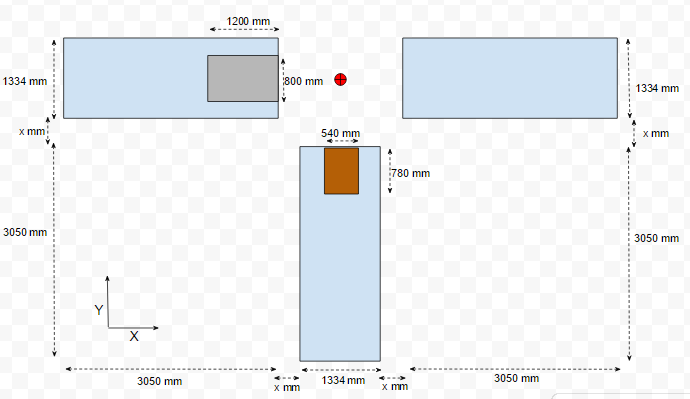
\includegraphics[width=\textwidth]{Description_de_la_solution/Layout.png}
		\caption{Layout a priori de la cellule}
		\label{fig:Layout}
	\end{center}
\end{figure}

Pour le rayon minimal, on considère que les convoyeurs se touchent, c’est-à dire, $x = 0$ $ mm $. De cette façon, avec le robot équidistant des convoyeurs (le point rouge), le rayon d’action du robot peut être calculé comme suit:
\begin{itemize}
\item On met le robot au milieu de la hauteur de la couche de cartons, ce qui correspond à trois cartons ($3 \times 350 = 1050$ $ mm $ par rapport aux convoyeurs);
\item Convoyeurs de palettes: il est aligné au robot dans l’axe Y et la distance dans l’axe X est $540 + 540/2 + 1334/2 = 1477$ $ mm $. Le rayon total $d=\sqrt{1477^2 + 1050^2} = 1812.19$ $ mm $.
\item Convoyeur de cartons: il est aligné au robot dans l’axe X, et la distance dans l’axe Y est $1334/2 + 780/2 = 1057$ $ mm $. Le rayon total $d = \sqrt{1057^2 + 1050^2} = 1498.88$ $ mm $.
\end{itemize}
Alors, le rayon minimale est 1812.19 $ mm $. Dans la suite, on a la liste des robots qui satisfont ces critères et leurs caractéristiques.


\begin{table}[H]
\caption{ Robots qui satisfont les critères du problème}
\label{tab:Robots_qui_satisfont}
\centering
\begin{tabular}{c|c|c|c|c|c|c}	

	\textbf{Série} &	\textbf{Version}&	\textbf{Type}&	\textbf{Charge Max. ($ Kg $)}&	\textbf{Rayon ($ mm $)}&	\textbf{Axes}&	\textbf{Prix}\\
	\hline 
	R-1000&	iA&	80H&	80&	2230& 5& 45 000 \euro\\
	\hline 
	R-2000&	iB&	100H& 100&	2655& 5& 50 000 \euro	\\
	\hline
	M-410&	iB&	140H& 140&	2850&	5&	55 000 \euro	\\
	\hline
	M-410&	iC&	185&	185&	3143&	4&	55 000 \euro	\\
	\hline
	M-410&	iC&	315&	315&	3143&	4&	55 000 \euro	\\
	\hline
	M-410&	iB&	450&	450&	3130&	4&	-	\\
	\hline
	M-410&	iB&	700&	700&	3143&	4&	-	\\

\end{tabular} 
\end{table}
\pagebreak
Pour choisir un d'entre les robots qui satisfont les critères, on a fait l’analyse budgétaire des séries R-1000, R-2000 et M-410. Le R-1000iA/80H est le moins cher, alors on l’a choisi pour faire des tests de simulation dans le but d’analyser s’il répond bien à la cadence de production.
La cadence du convoyeur de carton est de 411 produits/heure, ce qui correspond à un carton toutes les 8.76 secondes. La distance entre le carton et la position la plus loin où le carton doit être déposé dans la palette est 2,776 $ m $, et alors la vitesse moyenne du robot pour mettre le carton dans la palette et retourner à la position initiale doit être supérieur à 0,64 $ m/s $, une vitesse qui semble raisonnable pour le robot.
On a simulé le robot toute en contrôlant le taux des cartons, et la vitesse du robot est vraiment suffisante. 

\mysubsection{Placement du robot et des \textit{fixtures}}

Les convoyeurs sont des éléments importants pour le fonctionnement de la cellule, puisqu’ils y apportent les cartons, et les emportent. Cependant, ils occupent une surface considérable de la cellule. Alors, on a commencé l’optimisation de la surface pour trouver une bonne disposition des convoyeurs dans la cellule. On a considéré que la largeur minimale des convoyeurs de palette est la largeur des palettes (800 $ mm $) et la largeur minimale du convoyeur de cartons est la largeur des cartons (540 $ mm $). On a ajouté à ces valeurs une marge de sécurité.
Le placement des \textit{fixtures} qui nous semble permettre de réduire le plus la surface est montrée dans les images suivantes.

\begin{figure}[H]
	\begin{center}	
		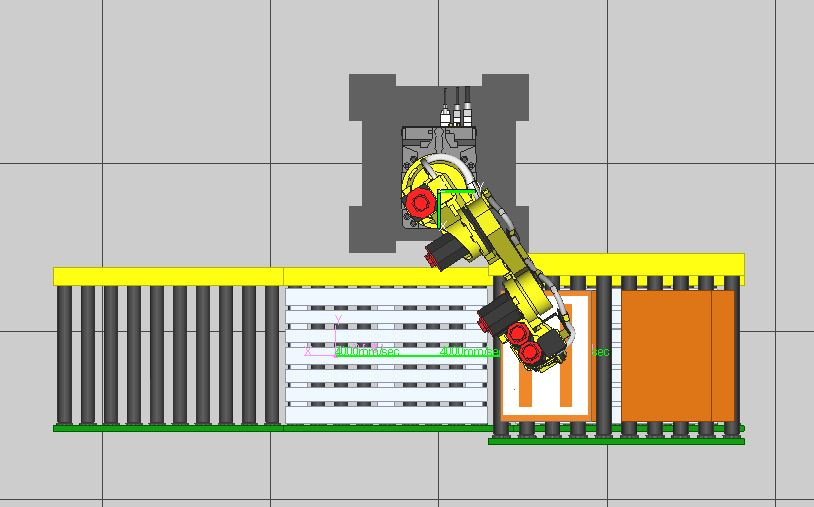
\includegraphics[width=\textwidth]{Description_de_la_solution/Vue_1.jpg}
		\caption{Vue du dessus de la cellule robotique}
		\label{fig:Vue_1}
	\end{center}
\end{figure}
\pagebreak
\begin{figure}[H]
	\begin{center}	
		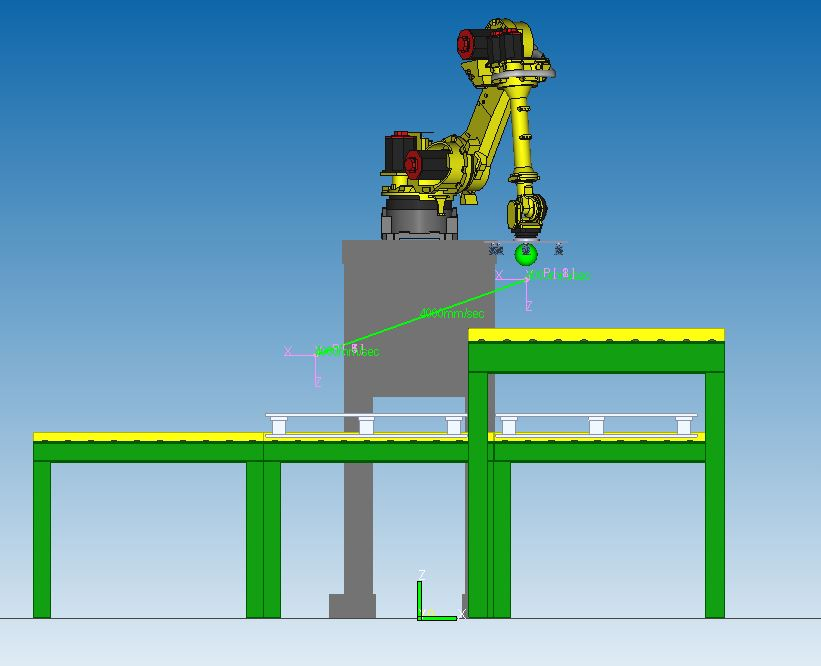
\includegraphics[width=\textwidth]{Description_de_la_solution/Vue_2.jpg}
		\caption{Vue frontale de la cellule robotique}
		\label{fig:Vue_2}
	\end{center}
\end{figure}


Pour choisir cette configuration, on a résolu la limitation suivante: les emplacements où les cartons et les palettes sont posés sur le convoyeur et d’où les palettes sont prises doivent être inaccessible pour le robot, dans le but de garantir la sécurité de ceux qui vont les poser (un ouvrier ou une autre machine). C’est possible d’effectuer les opérations souhaitées avec un seul convoyeur de palettes qui fonctionne à un seul sens. \par De cette manière, on a besoin de trois zones dans le convoyeur: une pour poser les palettes vides, une empiler les cartons sur la palette par le robot et une autre pour prendre les palettes pleines. Avec cette disposition, la seule façon qu’on a trouvé pour réduire la surface occupée par des convoyeurs est en verticalisant les opérations. Il est possible de mettre le convoyeur de cartons sur la partie des convoyeurs de palette où le palettes vides sont placées. Pour ce faire, les normes de sécurité doivent être pris en compte, car des opérateurs peuvent travailler dans cette zone pour poser les palettes. Ces normes de sécurité seront discutées dans la section \ref{considerations}. 

Un avantage de cette solution est que, en plus d’être efficace par rapport à la disposition des convoyeurs, elle réduit aussi la distance entre les cartons et la position où ils doivent être déposés sur les palettes. Cela permet de réduire la surface de l’îlot occupé par la trajectoire du robot aussi bien que de réduire le temps d’empilage des cartons sur la palette.
Pour le robot, le plus efficace est le placer au milieu de sa zone de travail. Comme il doit empiler des cartons en 6 couches sur une palette, qui est sur un convoyeur, la zone de travail vertical du robot se prolonge du premier carton dans la palette jusqu’au sixième. Le milieu correspond alors à la hauteur du convoyeur de carton plus la hauteur de trois cartons: 2150 $ mm $. Expérimentalement, la meilleure hauteur qu’on a trouvé est 2250 $ mm $. Le robot est donc placé sur un piédestal.
Pour la position horizontale du robot, on a choisi le milieu du palette qui est en train d’être remplie avec les cartons, avec une distance horizontale 454 $ mm $ entre le centre du robot et le début du convoyeur de palettes.

\mysubsection{Trajectoire du robot}

Pour déterminer les points qui vont contrôler la trajectoire du robot, on n’utilise qu’un repère user. Ce repère est défini par rapport au centre de la base du robot, 2250 $ mm $ au dessous, ce qui correspond au sol. De cette façon, il était plus facile de déterminer les points, avec leur hauteur ‘globale’. La direction des axes est montrée dans les figures \ref{fig:Vue_1} et \ref{fig:Vue_2}.


Comme toutes les opérations du robot sont faites dans une même ligne en X, et tous les convoyeurs étant horizontales, un seul repère est suffisant.

Pour générer la trajectoire du robot, on n’utilise que deux positions fixées: les points $ P_1 $ et $ P_2 $. $P_1$ correspond à la position sur le milieu du carton qui arrive dans le convoyeur de cartons. $P_2$ correspond à la position sur le milieu du carton de la première couche qui remplit la palette, à gauche. $P_1$ et $P_2$ sont montrés dans la figure suivante. Tous les points de la trajectoire sont générés avec ces positions, en appliquant des offsets.

\begin{figure}[H]
	\begin{center}	
		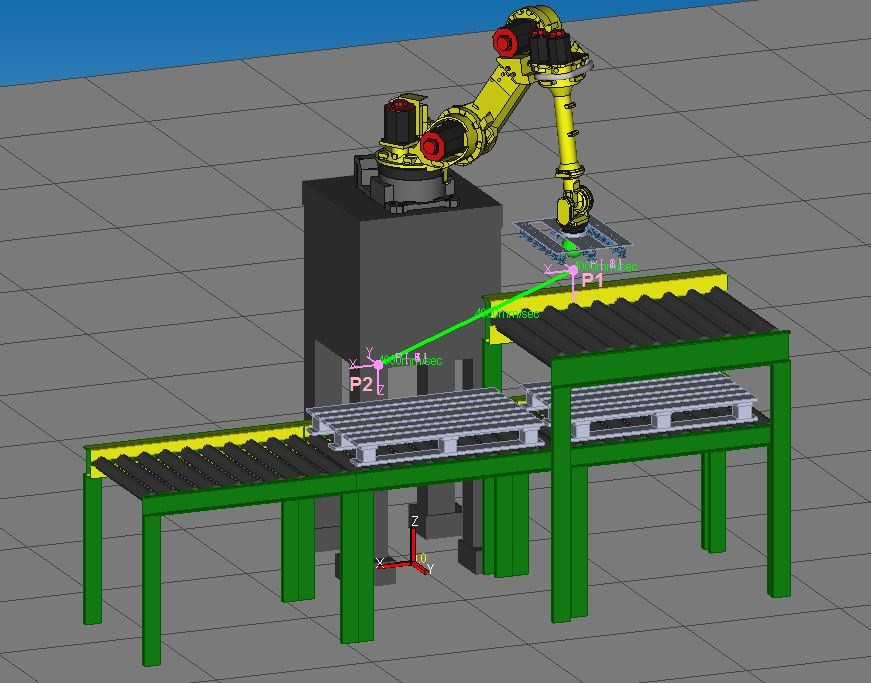
\includegraphics[width=\textwidth]{Description_de_la_solution/Pos.jpg}
		\caption{Positions de référence du programme du robot}
		\label{fig:Pos}
	\end{center}
\end{figure}

Pour générer des offsets pour la trajectoire, on utilise six points de référence PR. Dans le tableau \ref{tab:offsets}, il y a toutes les correspondances entre les PR qu’on a utilisé, leur fonction et leur valeur.

\begin{table}[H]
	\renewcommand{\tabularxcolumn}[1]{>{\small}m{#1}}
	\caption{Offsets utilisés dans le programme du robot}
		\label{tab:offsets}
		\begin{tabularx}{\textwidth}{>{\centering\arraybackslash}X|>{\centering\arraybackslash}X|>{\centering\arraybackslash}X}			
			\textbf{Point de référence}&
			\textbf{Fonction}&
			\textbf{Valeur (mm)}\\
			\hline			
			PR[1]&
			Point de départ du programme.&
			$P_1$ + (0, 0, 150)\\
			\hline			
			PR[2]&
			Distance verticale d’approche pour la prise des cartons.&
			(0, 0, 150)\\			
			\hline
			PR[3]&
			Distance verticale pour éviter les collisions du robot avec les cartons déjà positionnées lors qu’il enlève le carton du convoyeur de cartons.     &
			PR[2], si le robot est en train de remplir la première couche dans la palette,  sinon, (0, 0, PR[5,3] - 350)\\
			\hline			
			PR[4]&
			Déterminer la position du prochain carton à être déposé sur le palette.&
			(0, Yc, Zc), étant Yc égal 0 pour les cartons à gauche 600 à droite, et Zc = (i-1)*350,’ i‘ la couche du carton\\
			\hline
			PR[5]&
			Distance verticale d’approche pour la dépose des cartons.&
			PR[4] + PR[2]\\
			\hline
			PR[6]&
			Distance verticale pour éviter les collisions du robot avec les cartons déjà positionnées lors qu’il va déposer le carton dans la palette.   &
			PR[5] + (0, 0, 350)\\			
		\end{tabularx}
\end{table}

On a défini huit points pour maîtriser la trajectoire du robot. Ces points utilisent les offsets montrés avant et sont variables avec la position du carton à être déposé sur la palette. La figure \ref{fig:traj} montre la trajectoire du robot, en remarquant les points fixées. La tableau \ref{tab:points} explique la fonction de chaque point choisi.\par
On peut observer dans la tableau \ref{tab:points} qu’il n’y a que trois points de type FINE. Ces points correspondent aux emplacements où le robot doit prendre le carton (P[2]), déposer le carton (P[6]) et s’arrêter en attente pour le prochaine carton. Par conséquent, leur position doit être précisément respectée, et pour cela on utilise les points du type FINE. Les autres points sont utilisés pour bien fixer le profil de la trajectoire du robot, mais il n’a pas besoin de passer exactement sur eux. Pour cela on utilise les points CNT 100.\\
Tous les mouvements du robot sont du type \flq{}Linear\frq{}. Ce type de mouvement n’est pas le plus optimal par rapport à la vitesse du robot, mais de cette façon on limite les mouvements du robot à la zone sur le convoyeur de palettes, et on peut réduire plus la surface de l'îlot, ce qui est l’objectif principal du projet. Par rapport à la cadence du processus, les mouvements linéaires sont suffisants, et cette question est mieux explorée dans la section \ref{cadence}.
La figure \ref{fig:mov} montre toute la trajectoire du robot pour remplir une palette avec six couches de deux cartons.
\pagebreak


\begin{table}[H]
	
	\caption{Points utilisés dans la trajectoire du robot}
	\label{tab:points}
	\begin{tabularx}{\textwidth}{>{\centering\arraybackslash}X|>{\centering\arraybackslash}X|>{\centering\arraybackslash}X|>{\centering\arraybackslash}X}			
		
		\textbf{Point}&	\textbf{Fonction}&	\textbf{Valeur}&	\textbf{Type}\\
		\hline		
		P[1]&	Point d’approche pour la prise&	$P_1$ + PR[2]&	CNT 100\\
		\hline		
		P[2]&	Point de prise d’un carton&		$P_1$&
		FINE\\
		\hline		
		P[3]&
		Point intermédiaire pour aller au convoyeur de palettes sans collision avec la pile de cartons &
		$P_1$ + PR[3]&
		CNT 100\\
		\hline		
		P[4]&
		Point intermédiaire sur le convoyeur de palettes sans collision avec la pile de cartons& 
		$P_2$ + PR[4] + PR[6]&
		CNT 100\\
		\hline		
		P[5]&
		Point d’approche pour la dépose&
		$P_2$ + PR[4] + PR[5]&
		CNT 100\\
		\hline
		P[6]&
		Point de dépose d’un carton&
		$P_2$ + PR[4]&
		FINE\\
		\hline
		P[7]&
		Point intermédiaire pour retourner sur le convoyeur de cartons sans collision avec la pile de cartons&
		$P_2$ + PR[4] + PR[6]&
		CNT 100\\
		\hline
		P[8]&
		Point d’attente pour un autre carton qui arrive sur le convoyeur de cartons&
		$P_1$ + PR[3]&
		FINE\\
	\end{tabularx}
\end{table}



\begin{figure}[H]
	\begin{center}	
		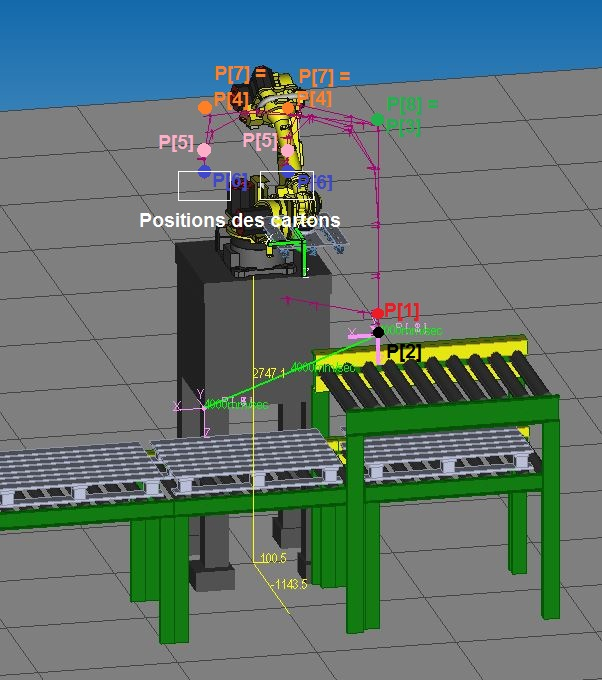
\includegraphics[height=.45\textheight]{Description_de_la_solution/traj.jpg}
		\caption{Trajectoire réalisée par le robot}
		\label{fig:traj}
	\end{center}
\end{figure}

\begin{figure}[H]
	\begin{center}	
		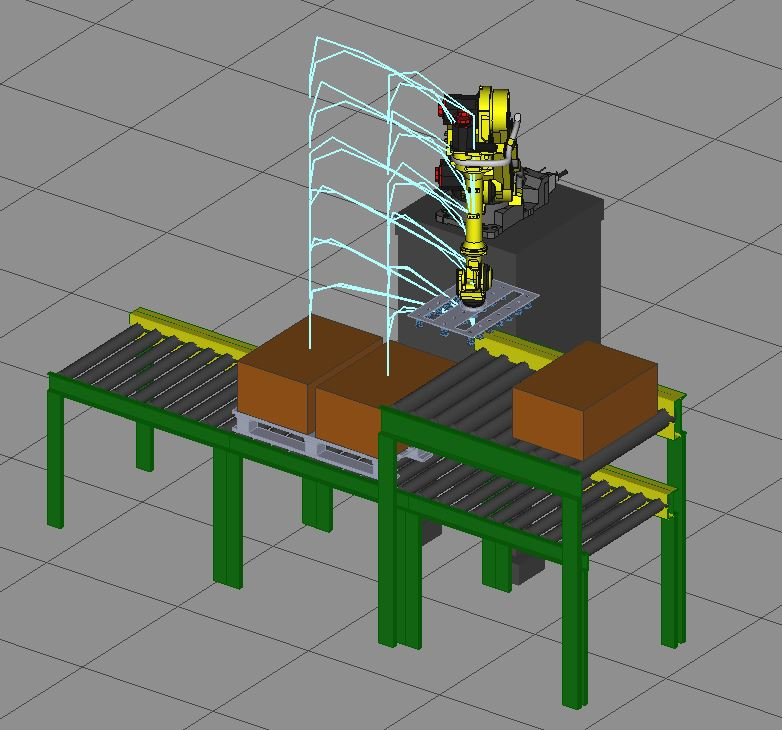
\includegraphics[width=\textwidth]{Description_de_la_solution/mov.jpg}
		\caption{Trajectoire du robot pour remplir une palette}
		\label{fig:mov}
	\end{center}
\end{figure}











\mysubsection{Considérations relatives à la sécurité opérationnelle}
\label{considerations}
Comme décrit dans la section \ref{cadre}, les mesures de sécurité représentent une partie essentielle de notre solution. Dans le contexte de la sécurité on proposera l’utilisation des fonction DCS, disponibles pour les robots FANUC. Pour nous aider à concevoir et dimensionner les systèmes de sécurité nous utiliserons la norme ISO 13849-1, qui concerne les parties relatives à la sécurité d’un système de commande (SRP/CS) et classifie les risques en termes de Performance Level, comme décrit succinctement dans la figure \ref{fig:X}.
\par
D’abord il faut identifier les sources de risque présentes dans la cellule. Les palettes sont introduites dans le convoyeur, aussi bien que enlevés, par des chariots élévateurs. Cette interaction se produit à l’intérieur de l’enveloppe de travail du robot, et donc il y a le risque des blessures graves, en plus cet accès est assez fréquent.
\newpage

\begin{figure}[H]
	\begin{center}	
		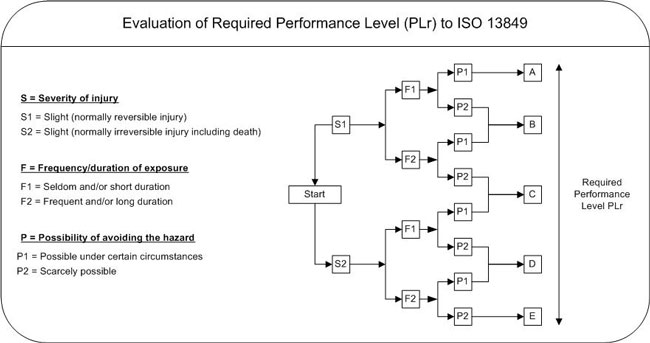
\includegraphics[width=\textwidth]{Description_de_la_solution/X.png}
		\caption{Évaluation du niveau PLr. Source: \cite{siteeller}}
		\label{fig:X}
	\end{center}
\end{figure}

 

Le risque est particulièrement grave dans l'espace entre les deux convoyeurs. Un autre risque est trouvé dans la période de maintenance pendant laquelle le technicien sera en contact direct avec le robot. Le processus de maintenance doit se produire souvent pour garantir le bon fonctionnement du robot et augmenter sa durée de vie. Le dernier risque associé à l'opération du robot est la chute des objets, particulièrement les cartons, ce qui est un risque constant dans l’opération de la cellule. Les évaluations des risques en termes de Performance Level requis sont présentées dans le tableau \ref{tab:Performance}.

\begin{table}[H]
	\caption{Performance Level Requis}
	\label{tab:Performance}
	\begin{tabularx}{\textwidth}{>{\centering\arraybackslash}X|>{\centering\arraybackslash}X|>{\centering\arraybackslash}X|>{\centering\arraybackslash}X|>{\centering\arraybackslash}X}
		\textbf{Source de Risque}&
		\textbf{S}&
		\textbf{F}&
		\textbf{P}&
		\textbf{PLr}\\
		\hline
		Accès des palettes&
		S2&
		F2&
		P1&
		PLd\\
		\hline
		Maintenance&
		S2&
		F1&
		P1&
		PLb\\
		\hline
		Chute d’objets&
		S1&
		F2&
		P1&
		PLb\\
	\end{tabularx}
\end{table}

Avant tout, pour éviter la chute des objets et empêcher l’entrée de personnel non autorisé il suffit de mettre en place une barrière autour de la cellule. La barrière doit être plus haute que la pile de cartons, dans la solution on a fixé la hauteur comme 4,2 $ m $.
Des panneaux  \flqq Ne pas franchir\frqq{}  pourront être apposés sur l’ensemble des barrières de manière lisible pour plus de sécurité.
\par
Afin de réduire le risque entre les deux convoyeurs on propose de fixer la barrière au convoyeur supérieur de façon que le robot n’ait pas accès direct aux opérateurs qui déposent les palettes, comme montré dans la figure \ref{fig:Detail_de_la_barriere}.

\pagebreak
\begin{figure}[H]
	\begin{center}	
		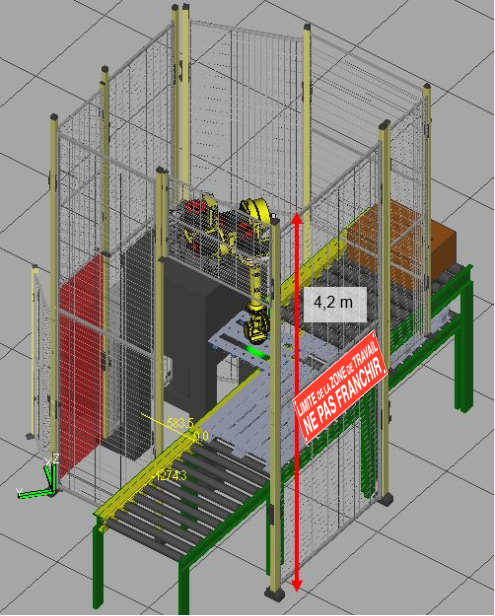
\includegraphics[height=.4\textheight]{Description_de_la_solution/hauteur.png}
		\caption{Cellule robotique avec les barrières}
		\label{fig:hauteur}
	\end{center}
\end{figure}



\begin{figure}[H]
	\begin{center}	
		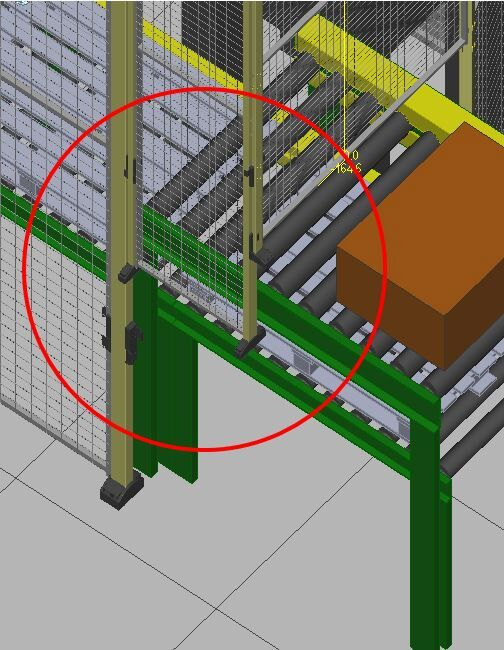
\includegraphics[height=.4\textheight]{Description_de_la_solution/Detail_de_la_barriere.png}
		\caption{Détail de la barrière fixé au convoyeur supérieur}
		\label{fig:Detail_de_la_barriere}
	\end{center}
\end{figure}	
\pagebreak
Malgré les barrières, les accès et la maintenance ne sont pas encore sécurisés. Pour répondre aux risques évalués comme PLd on utilisera la fonction \textit{Cartesian Position Check}  du DCS, et cette fonction garantit que dans le cas où le robot (ou le User Model du outil + carton) touche la limite de la région DCS la puissance du robot sera coupé immédiatement (power-off stop). La région permise du DCS est définie par cinq points comme on peut voir dans la figure \ref{fig:Points_de_la_region}. 


\begin{figure}[H]
	\begin{center}	
		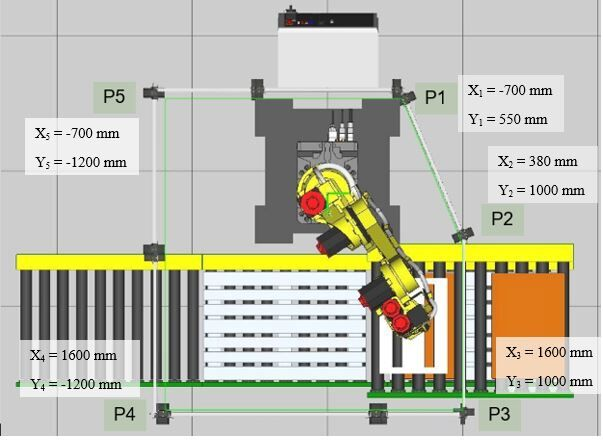
\includegraphics[width=\textwidth]{Description_de_la_solution/Points_de_la_region.png}
		\caption{Points de la région du Cartesian Position Check}
		\label{fig:Points_de_la_region}
	\end{center}
\end{figure}


La région externe à la barrière est sécurisé, ce qui réduit le risque expérimenté par les opérateurs. Le dernier risque qu’on doit traiter est, finalement, la maintenance, et pour ça on propose d’utiliser des interrupteurs de verrouillage dans la porte d’entrée de la cellule, qui coupent la puissance du robot lorsque la porte est ouverte, au moyen des entrées de sécurité du DCS (Fence input). 

\newpage
\mysubsection{Entrées et sorties du robot}

Pour bien synchroniser le mouvement du robot avec les autres éléments mobiles de la cellule, on a besoin d’utiliser les entrées et sorties numériques du robot. La tableau \ref{tab:in/out} décrit les signaux utilisés.

\begin{table}[H]
	\caption{Entrées et sorties numériques utilisées}
	\label{tab:in/out}
	\begin{tabularx}{\textwidth}{>{\centering\arraybackslash}X|>{\centering\arraybackslash}X|>{\centering\arraybackslash}X}
		
		\textbf{Nom}&
		\textbf{Type}&
		\textbf{Fonction}\\
		\hline
		DO[3]&
		Sortie&
		Activer le convoyeur pour apporter la palette pleine à la zone de déchargement. Est activé lorsque le robot finit de remplir une palette et désactivé lorsque la palette arrive dans la zone de déchargement.\\
		\hline
		
		DO[6]&
		Sortie&
		Activer le préhenseur à vide.\\
		\hline
		DI[1]&
		Entrée&
		Avertir le robot qu’il y a un carton disponible dans la région de prise.\\
		\hline
		DI[4]&
		Entrée&
		Avertir le robot qu’il y a une palette dans la position de chargement.\\
	\end{tabularx}
\end{table}

Pour que les DI soient générés, on a besoin de deux capteurs: un sur le convoyeur de cartons et un autre sur le convoyeur de palette. Le DO du robot doit contrôler le fonctionnement d’une partie du convoyeur de palettes.
Il y a d’autres signaux qui doivent être mesurés/générés  pour contrôler la cellule. Ces signaux sont montrés dans le tableau \ref{tab:signaux}, avec les noms qu’on a utilisés dans la simulation.

\begin{table}[H]
	\caption{Signaux externes pour contrôler la cellule}
	\label{tab:signaux}
	\begin{tabularx}{\textwidth}{>{\centering\arraybackslash}X|>{\centering\arraybackslash}X|>{\centering\arraybackslash}X}
		
		\textbf{Nom}&
		\textbf{Type}&
		\textbf{Fonction}\\
		\hline
		DO[2]&
		Signal de contrôle&
		Apporter les palettes vides à la position de chargement. Est activé si DI[3] = ON et DI[4] = OFF (il y a une palette vide et il n’y pas une palette en cours de remplissage).\\
		\hline
		DO[5]&
		Signal de contrôle&
		Apporter les cartons qui arrivent sur le convoyeurs de cartons à la positions de prise du robot. Est activé si DI[1] = ON et DI[2] = OFF (il y a un carton sur le convoyeur de cartons mais il n’y a pas un carton dans la position de prise). \\
		\hline
		DI[2]&
		Capteur&
		Avertir qu’il y a un carton qui arrive sur le convoyeur de carton.\\
		\hline
		DI[5]&
		Capteur&
		Avertir que la palette est arrivée dans la zone de déchargement.\\		
	\end{tabularx}
\end{table}




\newpage
On peut voir pour ces signaux que le convoyeur de palettes doit permettre leur activation par zone.
Il y en a aussi d’autres entrées/sorties dans notre programme Roboguide que ne sont utiles que pour contrôler la simulation.



\mysubsection{Programmation du robot}

Le programme qui contrôle le robot est composé globalement de deux fonctions. La première, qui s’appelle \textbf{MAIN}, est la fonction principale du programme. Dans cette fonction, on déclare et initialise toutes les variables du programme, les positions $P_1$ et $P_2$ et tous les points de référence (PR). On initialise aussi les sorties du robot (DO) et le payload. Cette fonction démarre trois boucles: une pour répéter les mouvements du robot à chaque palette vide qui arrive; une pour répéter la prise et dépose des cartons dans toutes les six couches sur la palette; et une pour répéter les mouvements de prise et dépose des cartons à droite et à gauche d’une même couche. \\
Pour faire les mouvements, la fonction \textbf{Prisedepose\_Conv} est appelée. Elle vérifie aussi les conditions des entrées (s’il y a un carton à prendre ou une palette pour déposer les cartons) pour mettre le robot en attente, lorsqu’il est nécessaire.
La fonction \textbf{Prisedepose\_Conv} déclare les points de mouvement du robot (P) et change leur valeur à chaque position sur la palette où le carton doit être déposé. Elle contrôle le mouvement du robot grâce à des points et contrôle aussi la prise et la dépose des cartons.
\par Dans le fichier Roboguide fourni avec la solution, il y a aussi d’autres fonctions dans le programme, mais ces fonctions ne sont utiles que pour la simulation.
Pour obtenir une simulation plus compatible avec la réalité, il faut ajouter les masses et les inerties des objets (carton et préhenseur) au programme de simulation, ce qui est fait par la déclaration du PAYLOAD. De cette façon, le logiciel les prendra en compte pour déterminer les efforts et la vitesse du robot. On aura une mesure plus précise du débit de la cellule. De plus, la programmation du PAYLOAD dans le programme TPE améliore les performances du robot et sa durée de vie.
Quelques autres détails ont été nécessaires pour générer et synchroniser le mouvement des objets dans la simulation, de manière à ce qu’elle semble plus réaliste. De cette façon, on a pu mesurer le débit de production pour le comparer avec l’antérieur. Les résultats sont détaillés dans la section \ref{cadence}.






